\chapter{TECNOLOGIAS E FERRAMENTAS UTILIZADAS}
\label{cap:TECNOLOGIAS-E-FERRAMENTAS-UTILIZADAS}


\section{Unity 3D – Ambiente de Desenvolvimento}
\label{sec:Unity-3D---Ambiente-de-Desenvolvimento}

Unity é uma ferramenta com múltiplas utilidades na qual permite o usuário a desenvolver desde um jogo simples até de um de última geração.

Segundo o próprio site onde é fornecida a ferramenta informa que o Unity é um motor de desenvolvimento integrado que fornece uma funcionalidade pioneira para criação de jogos e outros conteúdos interativos. Poderá utilizar o Unity para montar sua arte e recursos em cenas e ambientes; adicionar física, editar e testar simultaneamente seu jogo e, quando preparado, publicar em suas plataformas escolhidas, tais como computadores fixos, a rede, iOS, Android, Wii, PS3 e Xbox 360. 

O Unity suporta três linguagens de programação que são Boo, JavaScript e o C\#, esta última sendo utilizada para desenvolvimento do jogo Caapora. O Unity também possui módulos que podem ser instalados possibilitando o desenvolvimento sem linha de código. \cite{unt}
Na figura 15 é demonstrado o uso da Engine Unity 3D para o desenvolvimento do jogo. 



	\begin{figure}[h!]
		\centering
		\Caption{\label{fig:exemplo-1} Uso da engine Unity 3D para desenvovlvimento do jogo Caapora}	
		\UECEfig{}{
			\fbox{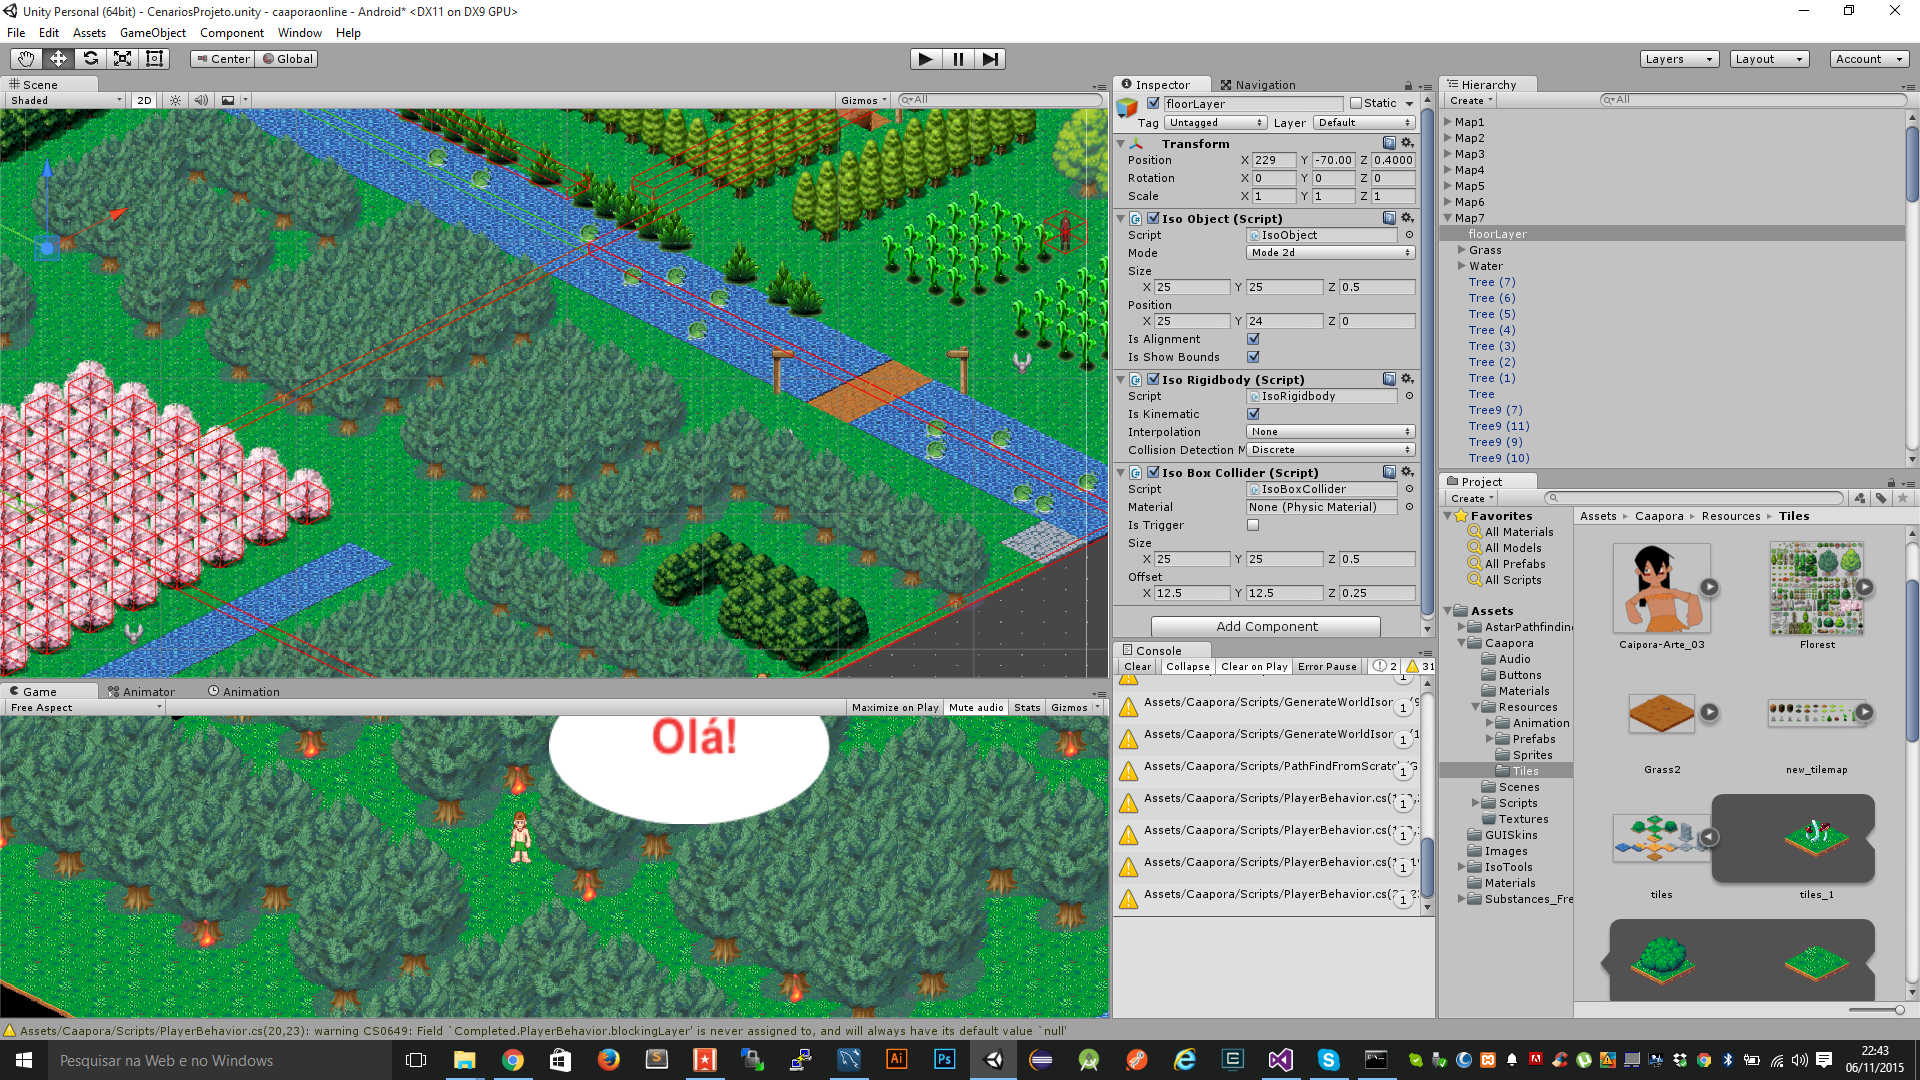
\includegraphics[width=10cm]{figuras/Unity}}
		}{
			\Fonte{Elaborado pelo autor}
		}	
	\end{figure}
	
Umas das principais vantagens de se utilizar o Unity é a possibilidade de desenvolver o jogo uma única vez e poder utiliza-lo em mais de 10 plataformas diferentes sem as necessidades de alterar o produto inicial. 
Algumas destas plataformas são: iPads, PC e iPhone. \cite{unt}

\subsection {Scene}

\textit{Scene} (traduzido do inglês livre: cena) é a parte mais importante dentro do jogo, pois cada uma representa uma fase dentro do jogo. Essa cena é constituída de vários objetos chamados de \textit{Gameobject}, que são recipientes onde pode ser agregados componentes.

Um \textit{gameobject} possui por padrão um componente chamado \textit{transform}, que tem como objetivo definir a posição, a rotação e a escala do objeto, ou seja sem ele o objeto não existiria dentro do jogo.
Na figura 16 temos o \textit {gameobject} do \textit {Player} acompanhado do componente \textit {transform}. \cite{unt}

\begin{figure}[h!]
		\centering
		\Caption{\label{fig:exemplo-1} Gameobject do Player}	
		\UECEfig{}{
			\fbox{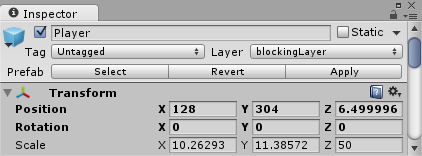
\includegraphics[width=10cm]{figuras/GameObject}}
		}{
			\Fonte{Elaborado pelo autor}
		}	
	\end{figure}


\section{Linguagem de programação C\#}
\label{sec:Linguagem-de-programação-Csharp}

C\# é uma linguagem elegante e de tipos protegidos, orientada a objeto e que permite aos desenvolvedores construírem uma variedade de aplicações seguras e robustas, compatíveis com o .NET Framework. É possível usar C\# para criar muito aplicativos de cliente do Windows, serviços Web XML, componentes distribuídos, aplicativos de cliente-servidor, aplicativos de banco de dados, e muito mais. 

O Visual C\# fornece um editor de códigos avançado, designers de interface de usuário convenientes, depurador integrado, e muitas outras ferramentas para facilitar o desenvolvimento de aplicativos baseados na linguagem C\# e no .NET Framework. 

A linguagem C\# foi desenvolvida pela Microsoft para ser um farmework .NET. 
O C\# é similar ao C++ e Java, sendo também uma linguagem fortemente tipada, orientada a objeto, portanto suporta heranças, polimorfismo e encapsulamento. 
Algumas características desta linguagem são: 

\begin{alineascomponto}
	\item Controle de versão: cada assembly gerado, seja como EXE ou DLL, tem informação sobre a versão do código. 

	\item Orientada a objetos: em C\#, qualquer variável tem de fazer parte de uma classe.  

	\item Linguagem gerenciada: todo gerenciamento de memória é feito pelo \textit{runtime} via GC (GarbageColletor), e não diretamente pelo programador, reduzindo assim as chances de cometer erros comuns.
\end{alineascomponto}
\cite{mcs}

\section{Adobe Illustrator CC}
\label{sec:Adobe-Illustrato-CC}

A Adobe Illustrator CC é um software de gráficos vetoriais padrão do setor, usado em todo o mundo por designers de todos os tipos que querem criar gráficos digitais, ilustrações e tipografia para todos os tipos de mídia: impressão, web, interativa, vídeo e móvel. \cite{adb}

O software Adobe Illustrator foi utilizado para a criação de \textit{sprites} dos personagens, como pode ser visto na figura 17 e outras funcionalidades utilizadas no Capoora Games.

\begin{figure}[h!]
		\centering
		\Caption{\label{fig:exemplo-6} Utilização do Adobe Illustrator CC no jogo Caapora}	
		\UECEfig{}{
			\fbox{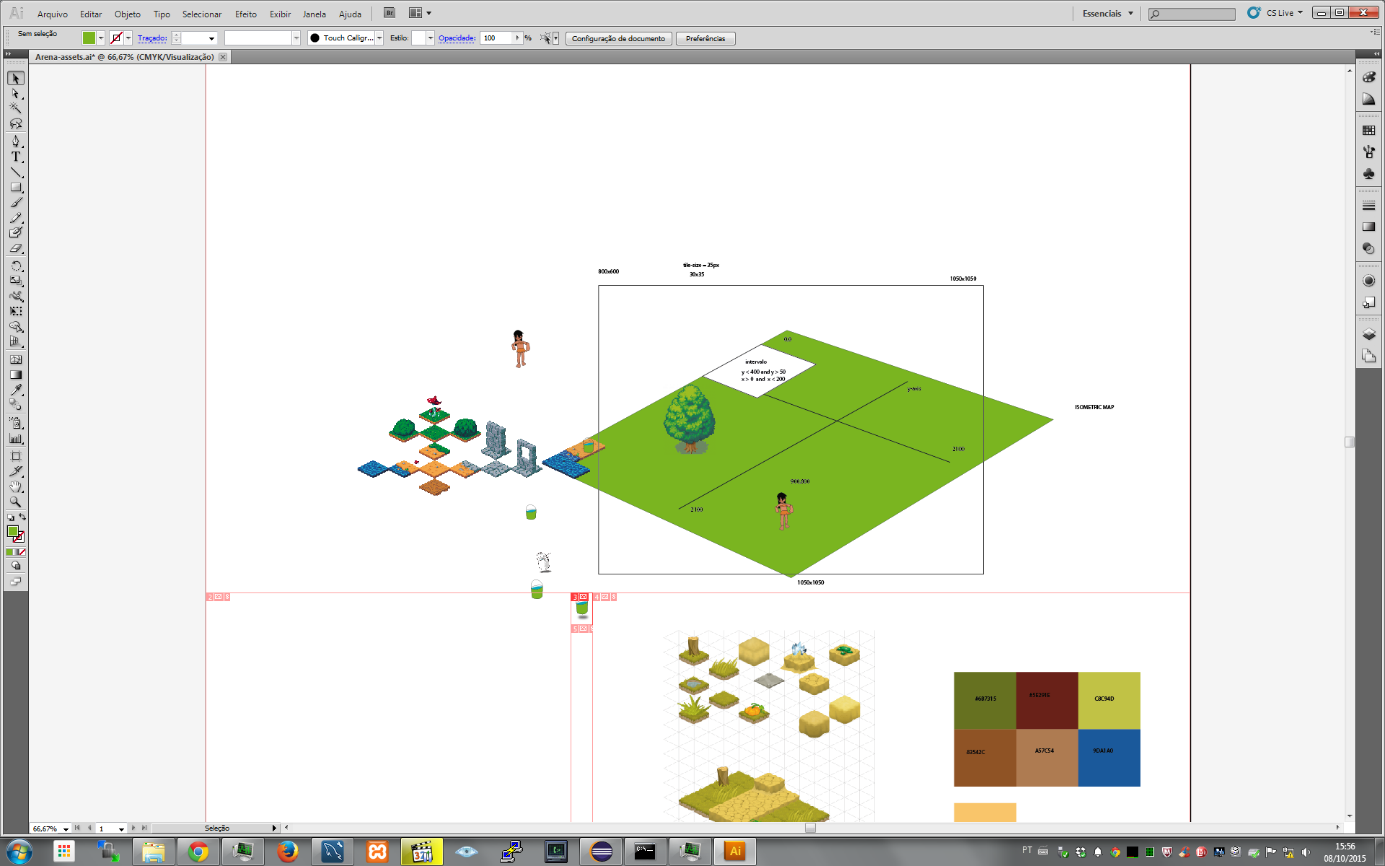
\includegraphics[width=10cm]{figuras/AdobeICC}}
		}{
			\Fonte{Elaborado pelo autor}
		}	
	\end{figure}
	
	\section{Visual Studio 2015}
\label{sec:Visual Studio 2015}

Visual Studio é um ambiente de desenvolvimento da Microsoft na qual permite desenvolver aplicativo para plataformas WEB, Windows, Mac e Linux. É uma ferramenta direcionada para desenvolver em linguagem de programação C\# e o \textit{framework} .NET.

Segundo o propio site da Visual Studio, a empresa define a ferramenta como: " Um ambiente de desenvolvimento integrado e sofisticado para criação de aplicativos impressionantes para Windows, Android e iOS, de aplicativos Web modernos e serviços de nuvem. " 

Uma grande vantagem em se utilizar o Visual Studio 2015 é permitir o desenvolvimento em multiplataforma e também a disponibilidade de variadas extensões, de PHP a serviços de jogos. \cite{vs}
